\documentclass[arhiv]{izpit}
\usepackage{times}
\usepackage{fouriernc}
\usepackage{tikz}
\renewcommand{\ttdefault}{txtt}

\begin{document}

\izpit{Programiranje I: 4.\ izpit}{27.\ avgust 2012}{
  Čas reševanja je 120 minut.
  Doseženih 100 točk šteje za maksimalno oceno.
  Veliko uspeha!
}

%%%%%%%%%%%%%%%%%%%%%%%%%%%%%%%%%%%%%%%%%%%%%%%%%%%%%%%%%%%%%%%%%%%%%%
\naloga[25 točk]

Mobilni operater poskuša svoje bazne postaje razporediti tako, da so med seboj razmaknjene vsaj 1000 m.
Sestavite funkcijo \verb|naloga1(sez)|, ki vrne \verb|True|, če so vse postaje v seznamu \verb|sez| dovolj razmaknjene, in \verb|False|, če obstajata postaji, ki sta si bliže kot 1000 m.
Postaje so predstavljene s koordinatami \verb|(x,y)|, izraženimi v metrih v kartezičnem koordinatnem sistemu (ukrivljenost Zemlje zanemarimo).

% Rešitev (ni preizkušena):

% def preblizu(lst):
%    d = 1000 # minimalna dovoljena razdalja
%    n = len(lst)
%    for i in range(0, n):
%        for j in range(i+1, n):
%            (x,y) = lst[i]
%            (u,v) = lst[j]
%            if (x - u) * (x - u) + (y - v) * (y - v) < d * d: return True
%    return False
%%%%%%%%%%%%%%%%%%%%%%%%%%%%%%%%%%%%%%%%%%%%%%%%%%%%%%%%%%%%%%%%%%%%%%
\naloga[25 točk]

\emph{Zadnji skupni prednik} dveh vozlišč v iskalnem drevesu je zadnje skupno vozlišče na poteh od korena do danih vozlišč (prvo skupno vozlišče je koren).
Tako je v drevesu
\[
  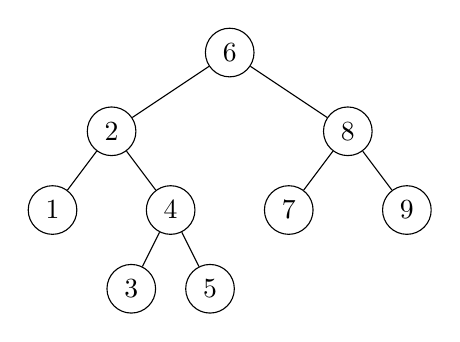
\begin{tikzpicture}[level distance=1cm,
    level 1/.style={sibling distance=3cm},
    level 2/.style={sibling distance=1.5cm},
    level 3/.style={sibling distance=1cm}
    ]
    \node[circle, draw] {6}
      child {node[circle, draw] {2}
        child {node[circle, draw] {1}}
        child {node[circle, draw] {4}
          child {node[circle, draw] {3}}
          child {node[circle, draw] {5}}
        }
      }
      child {node[circle, draw] {8}
      child {node[circle, draw] {7}}
        child {node[circle, draw] {9}}
      };
  \end{tikzpicture}
\]
vozlišče $2$ zadnji skupni prednik vozlišč $1$ in $5$, vozlišče $8$ pa zadnji skupni prednik vozlišč $8$ in $9$.

Razredu \verb|IskalnoDrevo| dodajte metodo \verb|naloga2(self,x,y)|, ki vrne zadnjega skupnega prednika vozlišč \verb|x| in \verb|y| v danem drevesu.
Časovna zahtevnost metode naj bo $O(k)$, kjer je $k$ dolžina poti od korena do iskanega zadnjega skupnega prednika.
Predpostavite lahko, da sta vozlišči \verb|x| in \verb|y| obe v drevesu.

%%%%%%%%%%%%%%%%%%%%%%%%%%%%%%%%%%%%%%%%%%%%%%%%%%%%%%%%%%%%%%%%%%%%%%
\naloga[30 točk]
Pri tej nalogi boste v \emph{Mathematici} risali večkotnike, včrtane enega v drugega.

\podnaloga[20 točk]
V \emph{Mathematici} sestavite funkcijo \verb|naloga3a[n_,k_]|, ki nariše \verb|k|
pravilnih \verb|n|-kotnikov, pri čemer naj bodo oglišča naslednjega večkotnika ravno na razpoloviščih stranic prejšnjega.

\begin{center}
  
\includegraphics[width=\textwidth]{naloga3a.eps} \\
  \quad  \verb|naloga3a[6, 3]|\hfill
  \verb|naloga3a[5, 8]|\hfill
  \verb|naloga3a[7, 4]|\hfill
  \verb|naloga3a[8, 12]|\hfill
\end{center}

\podnaloga[10 točk]
V \emph{Mathematici} sestavite funkcijo \verb|naloga3b[sez_]|, ki sprejme seznam \verb|sez| števil $n_1, \dots, n_k$ in nariše pravilne $n_j$-večkotnike ter njim včrtane krožnice, oglišča naslednjega večkotnika pa naj ležijo na včrtani krožnici prejšnjega.

\begin{center}
  
\includegraphics[width=\textwidth]{naloga3b.eps} \\
  \verb|naloga3b[{6, 5, 4, 3}]|\quad\quad\quad
  \verb|naloga3b[{4, 4, 4}]|\quad\quad\quad\quad
  \verb|naloga3b[{7, 5, 3}]|\quad
\end{center}

%%%%%%%%%%%%%%%%%%%%%%%%%%%%%%%%%%%%%%%%%%%%%%%%%%%%%%%%%%%%%%%%%%%%%%
\naloga[25 točk]

\emph{Izbor reda $n$} je podmnožica množice $\{1, 2, \dots, n\}$.
Vse izbore reda $n$ in moči $k$ lahko uredimo leksikografsko.
Na primer, izbori reda $5$ in moči $3$ so urejeni na sledeč način:
%
\[
  \{1, 2, 3\} < \{1, 2, 4\} < \{1, 2, 5\} < \{1, 3, 4\} < \{1, 3, 5\} <
  \{1, 4, 5\} < \{2, 3, 4\} < \{2, 3, 5\} < \{2, 4, 5\} < \{3, 4, 5\}
\]
%
Sestavite funkcijo $\mathtt{naloga4}(n, k, i)$, ki vrne $i$-ti izbor reda $n$ in moči $k$.
Izbor predstavite s seznamom, urejenim od najmanjšega do največjega števila.
Časovna zahtevnost funkcije naj bo $O(n)$.
Če je $i$ manjši ali enak $0$ oziroma večji od $n \choose k$, naj funkcija vrne \verb|None|.

\begin{verbatim}
>>> naloga4(5, 3, 1)
[1, 2, 3]
>>> naloga4(5, 3, 4)
[1, 3, 4]
>>> naloga4(5, 3, 7)
[2, 3, 4]
\end{verbatim}


\end{document}

